\documentclass{article}

\usepackage[preprint]{neurips_2025}

\usepackage[utf8]{inputenc}
\usepackage[T1]{fontenc}
\usepackage{hyperref}
\usepackage{url}
\usepackage{booktabs}
\usepackage{amsfonts}
\usepackage{amsmath}
\usepackage{microtype}
\usepackage{xcolor}
\usepackage[skip=3pt,font=small]{caption}
\usepackage{graphicx}

\graphicspath{{figures/}}

% Let floats take more of a page so tables do not get deferred past the text.
\renewcommand{\topfraction}{0.92}
\renewcommand{\bottomfraction}{0.85}
\renewcommand{\textfraction}{0.06}
\renewcommand{\floatpagefraction}{0.80}
\setlength{\textfloatsep}{10pt plus 2pt minus 2pt}
\setlength{\intextsep}{10pt plus 2pt minus 2pt}

% Tables and figures are generated by codes/report_assets.py so no number is typed by hand.

\title{Auditor ReAct: A Multi Agent ReAct System with Guardrails\\ for Fact Auditing, Math Reasoning and Code}

\author{%
  Ricardo A. Acu\~na-Villogas \quad Juan Aquino-Espinoza \quad Josu\'e Velo \\
  Universidad de Ingenier\'ia y Tecnolog\'ia (UTEC) \\
  \texttt{\{ricardo.acuna, juan.aquino, josue.velo\}@utec.edu.pe}
}

\begin{document}

\maketitle

\begin{abstract}
We build a system of three agents, a Researcher, a Fact Auditor and a Writer, coordinated by a LangGraph state graph on a local Qwen2.5 7B orchestrator quantised to 4 bits, with a FAISS index over WikiQA, GSM8K and MBPP, web search and Python execution, and compare it against a single step Naive RAG. On 50 dataset queries both systems reach 0.78 accuracy and disagree on only 8 of them, four each way, so the 95 percent interval of the difference, from $-0.12$ to $0.10$, contains zero; Naive RAG is also more faithful, 0.91 against 0.84. On 15 multi hop queries that need two documents and a calculation the multi agent system wins 6 to 0 ($p = 0.03$), 0.93 against 0.53. Per task, the faithfulness gap lives entirely in math and code, where answers state values computed with Python that no retrieved document contains. On code the Auditor verdict matches the test outcome in 15 of 15 queries, which makes it a reliable detector even when the Researcher cannot repair the function. With a 1.5B orchestrator the architecture loses to its own baseline, and moving the baseline from 1.5B to 7B wins 14 to 0: model size matters more than the number of agents.
\end{abstract}

\section{Introduction}

\noindent A Naive RAG retrieves once and generates once \citep{lewis2020rag}. It fails in three predictable situations: when the answer needs two documents and the single search returns one, when the question needs a calculation the model does from memory, and when the output is code that nobody ran. ReAct \citep{yao2023react} interleaves reasoning with tool calls, and an agent graph lets one agent investigate while another verifies. This report asks whether that extra machinery pays off, where, and at what cost.

\noindent We answer with one system and five configurations evaluated on the same queries: the full graph, the graph without its Auditor, the Naive RAG baseline, and both designs again with a 1.5B orchestrator. Because every configuration answers the same questions, we analyse the differences in pairs, question by question, and then read the failures one by one. The emphasis of the report is that analysis rather than the headline averages, which hide most of what happened.

\section{System}

\begin{figure}[!tb]
  \centering
  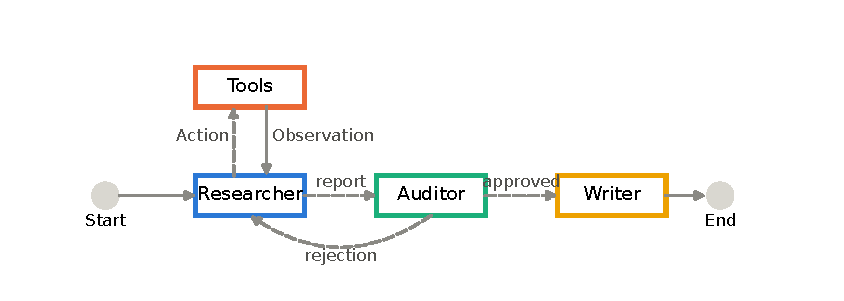
\includegraphics[width=0.78\linewidth]{fig1_grafo_agentes.pdf}
  \caption{Control graph compiled with LangGraph. Dashed edges are conditional: the Action and Observation loop between the Researcher and the tools, the Auditor rejection that returns the state to the Researcher, and the direct edge used when the Auditor is ablated.}
  \label{fig:graph}
\end{figure}

\paragraph{Control graph.}
The agents share a typed state (question, trace, retrieved contexts, report, number of rejections) in a LangGraph \citep{langgraph2024} state graph (Figure \ref{fig:graph}). The Researcher emits one step per turn in the format Thought, Action, Action Input; generation stops at the string Observation and the tool node injects the real observation, for at most six actions per attempt. Its final report goes to the Fact Auditor, which either approves it for the Writer or returns the state to the Researcher with a reason, at most twice. The Writer turns the approved report into the final answer and cites the identifiers of its sources. The three agents share one model and differ only in their system prompt.

\paragraph{Tools.}
buscar\_kb queries the local index and returns the three closest documents. buscar\_web uses DuckDuckGo and falls back to the Wikipedia API. ejecutar\_python runs code in a separate Python process with a 10 second limit. Any tool error, a misspelt tool name, code that prints nothing, a timeout or an unreachable search engine, is returned to the Researcher as an Observation instead of interrupting the graph, so the agent can correct itself in the next step (Appendix \ref{app:trace}).

\paragraph{Fact Auditor.}
The Auditor combines two guardrails. The deterministic one rejects a report with no tool evidence, and for code it runs the task asserts and returns the first one that fails. The semantic one asks the model to contrast the report with the observations and answer APPROVED or REJECTED with a reason.

\paragraph{Data processing.}
WikiQA \citep{yang2015wikiqa} ships as question and candidate sentence pairs; we group the sentences by article title, without duplicates and in their original order, so each article becomes one document (2\,811 documents, median 1\,065 characters). From GSM8K \citep{cobbe2021gsm8k} we index the 7\,473 training problems with their worked solution (median 511) and read the gold answer of test problems as the number after the \#\#\#\# marker, without thousands separators. From MBPP \citep{austin2021mbpp} we index the 474 task descriptions and reference functions of the train, validation and prompt splits (median 240) and keep the tests and setup code apart for the Auditor. Documents are short, so each is embedded whole, without chunking. The 10\,758 documents are encoded with all MiniLM L6 v2 \citep{reimers2019sbert}, normalised, and stored in a FAISS inner product index \citep{johnson2019faiss}, which on unit vectors is cosine similarity. The web application uses the same vectors quantised to int8.

\paragraph{Models and baseline.}
The orchestrator is Qwen2.5 7B Instruct \citep{qwen2025} in NF4 with double quantisation \citep{dettmers2023qlora}, about 6 GB of VRAM, with greedy decoding. The Naive RAG baseline retrieves the four documents closest to the question and answers in a single call with the same model.

\section{Experiments}

\paragraph{Queries and systems.}
With a fixed seed we sample 20 WikiQA test questions that have a correct sentence, 15 GSM8K test problems and 15 MBPP test tasks with their three asserts in the prompt; the GSM8K and MBPP queries are not in the index. To test the case that motivates the architecture we add 15 multi hop queries that ask for the years elapsed between two events described in two different WikiQA articles, with each year verified in the article text. The five systems are the multi agent graph, the graph without the Auditor and Naive RAG with the 7B orchestrator, and the multi agent graph and Naive RAG with Qwen2.5 1.5B.

\paragraph{Metrics.}
Following RAGAS \citep{es2024ragas}, Faithfulness is the fraction of atomic claims in the answer that the judge can infer from the context the system retrieved, computed in two steps (extract the claims, then verify each one). Answer Relevance is the mean cosine similarity between the question $q$ and three questions $\hat q_i$ the judge generates from the answer,
\begin{equation}
\mathrm{AR} = \frac{1}{3}\sum_{i=1}^{3} \cos\big(e(q),\, e(\hat q_i)\big).
\end{equation}
The judge is Phi 4 \citep{abdin2024phi4}, a different model family from the orchestrator, so the system never grades itself \citep{zheng2023judging}. Accuracy does not depend on the judge except on WikiQA: exact number on GSM8K, passed tests on MBPP, and judge correctness against the reference sentence on WikiQA. We also log seconds, LLM calls and tokens per query.

\paragraph{Pipeline.}
Four scripts communicate only through files: data preparation builds the corpus, the queries and the index; generation runs each system and writes one JSONL line per query with answer, trace, time per node and the objective metric; the judge adds Faithfulness, Answer Relevance and WikiQA correctness; a last script produces every table and figure of this report from those files. An interrupted run resumes at the last query, which mattered on a shared SLURM cluster with one RTX A6000. Paired differences are tested with a two sided sign test over the queries where two systems disagree, and with a 95 percent bootstrap interval (5\,000 resamples) for the accuracy difference.

\paragraph{Validating the evaluator.}
Before reading any result we audited the evaluation itself. The first judge generated questions in Spanish for English queries, which lowered Answer Relevance; the numeric extractor read citations such as [1] as the answer, which hid a perfect GSM8K score; and the parser turned a turn with no Action into an invalid action. All three were fixed before the final runs.

\section{Results and analysis}

\begin{table*}[!tb]
\centering
\caption{Results on the 50 dataset queries. Faithfulness and Answer Relevance from the judge; accuracy per task and overall; mean cost per query.}
\label{tab:main}
\footnotesize
\setlength{\tabcolsep}{3.5pt}
\begin{tabular}{lcccccccc}
\toprule
System & Faithful. & Answer Rel. & WikiQA & GSM8K & MBPP & Overall & Seconds & Calls \\
\midrule
Multi agent 7B & 0.84 & 0.68 & 0.80 & 1.00 & 0.53 & 0.78 & 44.6 & 6.2 \\
Naive RAG 7B & 0.91 & 0.72 & 0.85 & 1.00 & 0.47 & 0.78 & 4.8 & 1.0 \\
Multi agent, no Auditor 7B & 0.84 & 0.68 & 0.80 & 0.93 & 0.47 & 0.74 & 38.6 & 4.2 \\
Multi agent 1.5B & 0.47 & 0.44 & 0.65 & 0.60 & 0.13 & 0.48 & 49.4 & 6.8 \\
Naive RAG 1.5B & 0.78 & 0.64 & 0.60 & 0.73 & 0.13 & 0.50 & 3.8 & 1.0 \\
\bottomrule
\end{tabular}
\end{table*}


\paragraph{Main comparison.}
Table \ref{tab:main} gives the headline numbers. With the 7B orchestrator the multi agent graph and Naive RAG tie at 0.78 overall accuracy, Naive RAG scores higher on Faithfulness (0.91 against 0.84) and on Answer Relevance (0.72 against 0.68), and it is about nine times faster. The tie is explained by the queries rather than by the agents: the gold WikiQA document is among the top three retrieved for 99 percent of the questions (Appendix \ref{app:figures}), and the 7B model already solves every sampled GSM8K problem once it computes with Python. Only on MBPP, where tests can be executed before answering, does the graph come out ahead.

\begin{table}[!tb]
\centering
\caption{Paired comparison; 7B unless stated. A only and B only count the queries one system answers correctly and the other does not. Two sided sign test; the interval is a 95 percent bootstrap of the accuracy difference.}
\label{tab:paired}
\small
\begin{tabular}{lcccl}
\toprule
A vs B & $n$ & A only & B only & Test \\
\midrule
Multi agent vs Naive RAG, complex & 50 & 31 & 1 & $p < 0.001$ \\
Auditor vs no Auditor, complex & 50 & 4 & 2 & $p = 0.69$ \\
Multi agent vs Naive RAG, dataset & 50 & 4 & 4 & $p = 1.00$, CI $[-0.12, 0.10]$ \\
Auditor vs no Auditor, dataset & 50 & 3 & 1 & $p = 0.63$ \\
Naive RAG 7B vs 1.5B & 50 & 14 & 0 & $p < 0.001$ \\
Multi agent 1.5B vs Naive RAG 1.5B & 50 & 5 & 6 & $p = 1.00$ \\
\bottomrule
\end{tabular}
\end{table}


\paragraph{Are the differences real?}
Averages over 50 queries can hide that two systems fail on different questions. Table \ref{tab:paired} counts only the queries where two systems disagree. The multi agent graph and Naive RAG disagree on 8 of 50, four each way, and the bootstrap interval of the difference contains zero: on dataset queries the two designs are indistinguishable. The Auditor wins 3 to 1 against no Auditor, a direction worth keeping but not a conclusion at this sample size. Two effects are clear. On multi hop queries the graph wins 6 to 0 ($p = 0.03$). Moving Naive RAG from 1.5B to 7B wins 14 to 0, while at 1.5B the graph and its baseline are again level, so the orchestrator size moves accuracy far more than the architecture does.

\begin{table}[!tb]
\centering
\caption{Faithfulness and Answer Relevance per task, and share of multi agent queries that used web search.}
\label{tab:pertask}
\small
\begin{tabular}{lccccc}
\toprule
Task & \multicolumn{2}{c}{Faithfulness} & \multicolumn{2}{c}{Answer Rel.} & Web use \\
 & Multi & Naive & Multi & Naive & Multi \\
\midrule
WikiQA & 0.91 & 0.92 & 0.71 & 0.69 & 0.75 \\
GSM8K & 0.83 & 1.00 & 0.64 & 0.80 & 0.13 \\
MBPP & 0.74 & 0.82 & 0.68 & 0.68 & 0.13 \\
\bottomrule
\end{tabular}
\end{table}


\paragraph{Where the faithfulness gap comes from.}
Table \ref{tab:pertask} splits the metric by task. On WikiQA the two systems are equally faithful (0.91 and 0.92); the gap is on GSM8K (0.83 against 1.00) and MBPP (0.74 against 0.82). Reading the judge outputs shows why: the multi agent answer states totals computed with Python or describes the function it wrote, and none of that text is in the retrieved documents, so the judge marks it unsupported even when it is correct. The metric penalises what the system computed, not what it invented. A second behaviour adds cost without adding accuracy: the Researcher searched the web on 75 percent of WikiQA queries although the gold document was already in its first retrieval, which is also how a newer web figure ended up contradicting an older WikiQA reference.

\begin{table}[!tb]
\centering
\caption{The 50 complex queries: each needs two documents and one subtraction. Faithfulness and Answer Relevance from the judge.}
\label{tab:multihop}
\small
\begin{tabular}{lcccccc}
\toprule
System & Accuracy & Faithful. & Answer Rel. & Both docs & Seconds & LLM calls \\
\midrule
Multi agent 7B & 0.88 & 0.30 & 0.21 & 0.76 & 31.4 & 9.1 \\
Naive RAG 7B & 0.28 & 0.77 & 0.68 & 0.10 & 3.0 & 1.0 \\
Multi agent, no Auditor 7B & 0.84 & 0.28 & 0.21 & 0.76 & 23.0 & 5.8 \\
\bottomrule
\end{tabular}
\end{table}


\paragraph{Multi hop queries.}
Table \ref{tab:multihop} measures the case the architecture was built for. Every Naive RAG error happens when its single retrieval misses one of the two documents: it then asks for the missing data or guesses a year. The graph searches each event separately, retrieves both documents in 80 percent of the queries against 27 percent, subtracts with Python and nearly doubles the accuracy. The version without Auditor reaches the same accuracy in less time, so here the gain comes from decomposition and tools, not from the guardrail.

\paragraph{Error analysis.}
The 7B graph fails 11 of the 50 queries. Seven are MBPP tasks, and in all seven the Auditor found the failing assert and used both rejections without the Researcher managing to repair the function. Three are WikiQA answers that are partial or speculative against the reference sentence, for instance naming only Christianity when the reference says Christianity or Islam. The last is an outdated reference: WikiQA gives 1.5 billion dollars for the Yankee Stadium while the web gives 2.3. Naive RAG fails seven of these eleven as well, so they are the hard queries of the sample rather than errors introduced by the architecture.

\begin{table}[!tb]
\centering
\caption{Auditor verdict against the test outcome on the 15 MBPP queries (multi agent 7B).}
\label{tab:detector}
\small
\begin{tabular}{lcc}
\toprule
Final verdict & Passes tests & Fails tests \\
\midrule
Approved & 8 & 0 \\
Rejected twice & 0 & 7 \\
\bottomrule
\end{tabular}
\end{table}


\paragraph{The Auditor as a detector.}
Table \ref{tab:detector} crosses the final Auditor verdict with the test outcome on MBPP. Every function it approved passes the tests and every function it rejected twice fails them, 15 of 15. The Auditor does not always get the Researcher to fix the code, but its verdict is a reliable signal that could be shown to the user as unverified code instead of returning a function that fails. On GSM8K the picture is different: it rejected reports on 7 of 15 problems and changed the outcome on only one compared with no Auditor, so there it mostly adds time.

\begin{table}[!tb]
\centering
\caption{MBPP with an Auditor that rejects without returning the error (v1), one that returns the failing assert (v2), and no Auditor.}
\label{tab:auditor}
\small
\begin{tabular}{llccc}
\toprule
Model & Version & MBPP tests & Mean rejections & Seconds \\
\midrule
7B & No Auditor & 0.47 & 0.00 & 35.0 \\
7B & Auditor v1 & 0.47 & 1.93 & 82.1 \\
7B & Auditor v2 & 0.53 & 1.00 & 52.9 \\
1.5B & Auditor v1 & 0.13 & 1.60 & 74.6 \\
1.5B & Auditor v2 & 0.13 & 1.53 & 72.1 \\
\bottomrule
\end{tabular}
\end{table}


\paragraph{An Auditor must say what to fix.}
Our first Auditor rejected failing code with a generic reason, and the Researcher resubmitted the same report: it rejected 1.93 times per task, doubled the latency and did not improve on having no Auditor (Table \ref{tab:auditor}). Returning the failing assert and asking for a test run before reporting raised the passed tests from 0.47 to 0.53, halved the rejections and cut 29 seconds per task. With the 1.5B model neither version helps, because the Researcher cannot act on the feedback.

\paragraph{Orchestrator size.}
At 1.5B the multi agent graph is worse than its own Naive RAG. The Researcher ignores the rule of searching the local index first, invents data such as a non existent website, and its Auditor, the same small model, approves it; Faithfulness falls to 0.47, the lowest of all systems. The ReAct format and the guardrail both assume a model able to follow them.

\begin{figure}[!tb]
  \centering
  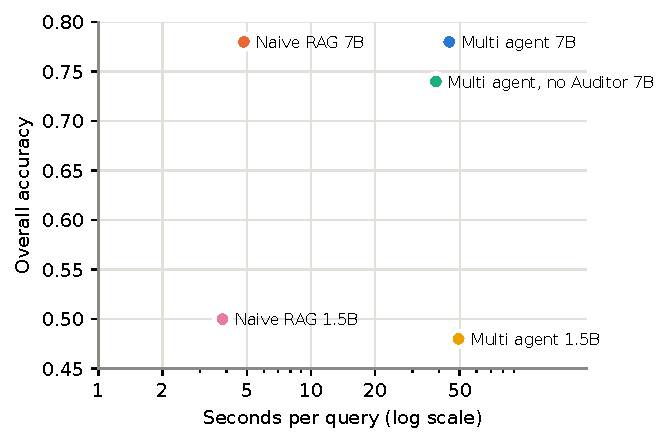
\includegraphics[width=0.48\linewidth]{fig4_calidad_vs_latencia.pdf}\hfill
  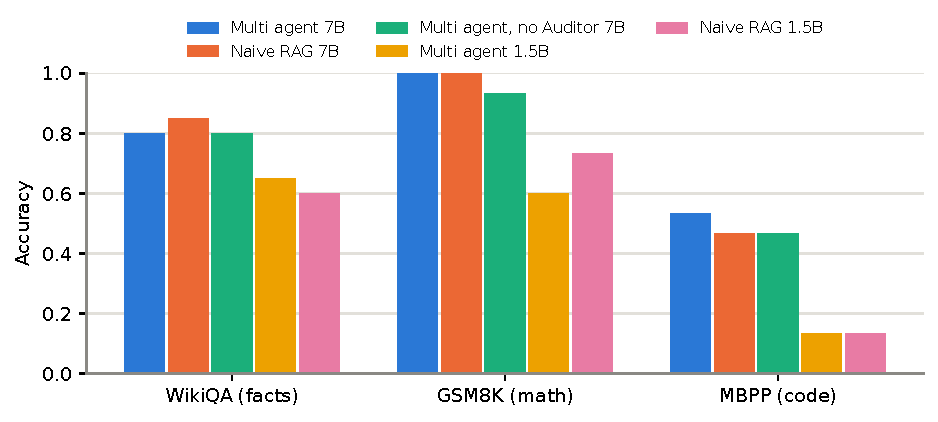
\includegraphics[width=0.5\linewidth]{fig3_acierto_por_tarea.pdf}
  \caption{Left: overall accuracy against seconds per query on a log scale; the graphs cost about an order of magnitude more time at equal or lower accuracy. Right: accuracy per task; the advantage of each design depends on whether the task allows checking something concrete.}
  \label{fig:cost}
\end{figure}

\paragraph{Cost.}
The graph costs 44.6 seconds per query against 4.8 for Naive RAG (Figure \ref{fig:cost}). Three quarters of that time is the Researcher generating thoughts (33.2 seconds); tools take 7.0 and the Auditor and Writer together 4.4 (Appendix \ref{app:figures}). Shrinking the model does not make the architecture cheaper, because the 1.5B graph spends twice as long in tools (15.2 seconds) and the Researcher is no faster.

\section{Conclusion}

\noindent On queries that a single retrieval already answers, three agents add no accuracy: the graph and Naive RAG disagree on 8 of 50 queries, four each way, and the single step is nine times faster and more faithful by the RAGAS measure, whose gap comes from computed values rather than invented ones. The graph pays off when the query is compound or verifiable: it wins 6 to 0 on multi hop queries, and on code its Auditor verdict predicts the test outcome in 15 of 15 cases, provided the feedback names what to fix. The orchestrator matters more than the agent count, so a production system should route: Naive RAG by default and the full graph when the query asks for several documents, a calculation or code. The web application released with the code exposes both modes with the live graph. The main limitation is sample size: with 50 and 15 queries, a single judge and a single seed, only two effects are statistically clear, and some WikiQA references are older than the web the agents consult.

\setlength{\bibsep}{1.5pt plus 0.3ex}
{\small
\renewcommand{\emph}[1]{#1}% no italics in the reference list
\bibliographystyle{plainnat}
\bibliography{refs}
}

\appendix

\section{Additional figures and tables}
\label{app:figures}

\begin{figure}[!htb]
  \centering
  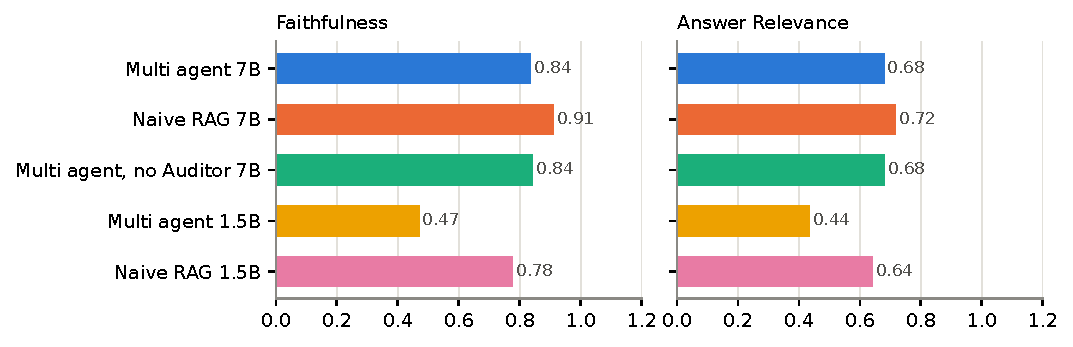
\includegraphics[width=0.85\linewidth]{fig2_ragas.pdf}
  \caption{Faithfulness and Answer Relevance per system. With 7B both designs are close; the 1.5B graph is the one that invents most.}
\end{figure}

\begin{figure}[!htb]
  \centering
  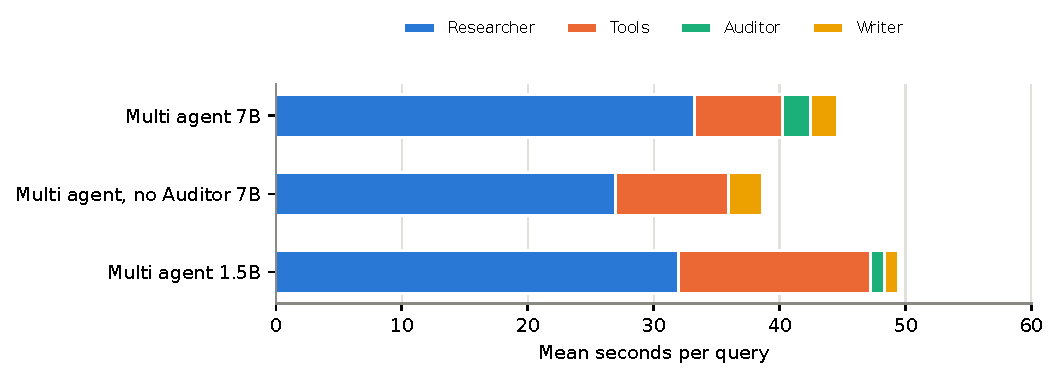
\includegraphics[width=0.52\linewidth]{fig5_latencia_por_agente.pdf}\hfill
  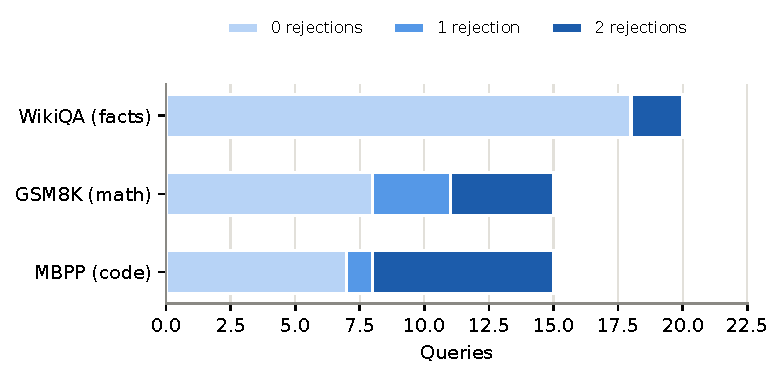
\includegraphics[width=0.44\linewidth]{fig6_rechazos_auditor.pdf}
  \caption{Left: mean seconds per query by node; the Researcher dominates. Right: Auditor rejections per task for the 7B graph; they concentrate on code and math, where something concrete can be checked.}
\end{figure}

\begin{figure}[!htb]
  \centering
  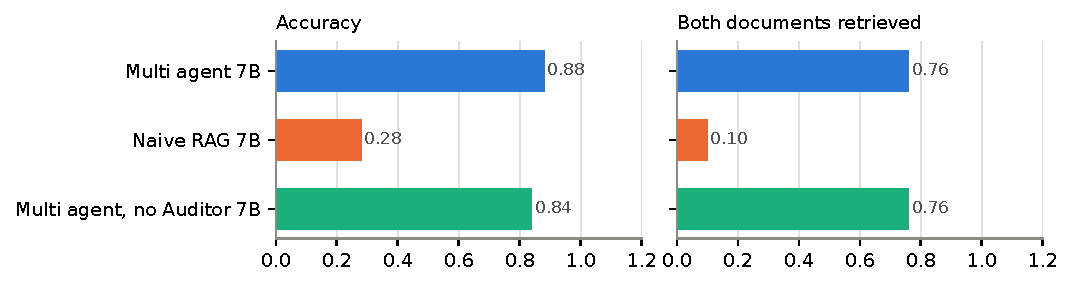
\includegraphics[width=0.85\linewidth]{fig8_multisalto.pdf}
  \caption{Multi hop queries: Naive RAG is only right when its single retrieval brings both documents.}
\end{figure}

\begin{table}[!tb]
\centering
\caption{Hit at k of the gold WikiQA document over the 243 test questions with an answer, and query time.}
\label{tab:retrieval}
\small
\begin{tabular}{lccccc}
\toprule
Embedder & Hit@1 & Hit@3 & Hit@5 & Hit@10 & ms per query \\
\midrule
paraphrase multilingual MiniLM L12 v2 & 0.82 & 0.89 & 0.93 & 0.95 & 17 \\
all MiniLM L6 v2 & 0.96 & 1.00 & 1.00 & 1.00 & 11 \\
bge small en v1.5 & 0.98 & 0.99 & 1.00 & 1.00 & 23 \\
\bottomrule
\end{tabular}
\end{table}


\begin{figure}[!htb]
  \centering
  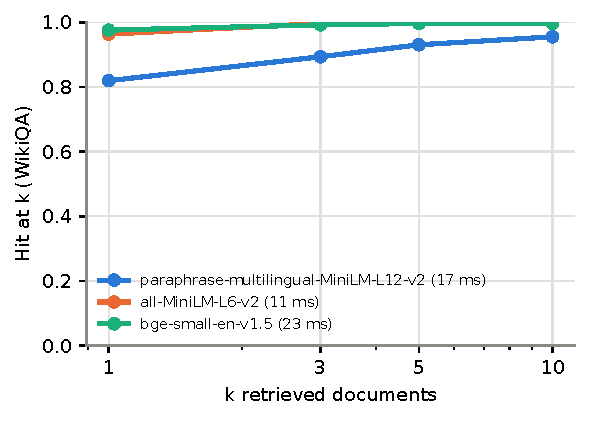
\includegraphics[width=0.45\linewidth]{fig7_recuperacion.pdf}
  \caption{Retrieval ablation (Table \ref{tab:retrieval}). The English models beat the multilingual one, and all MiniLM L6 v2 matches bge small at half its query time, so it is the embedder of the system.}
\end{figure}

\section{A ReAct trace from the evaluation}
\label{app:trace}

\noindent GSM8K query: Sarah spent 300 dollars on books at 15 dollars each and split them equally among her 4 children; how many books did each child get? The Researcher of the 7B graph produced:

\begin{enumerate}
  \item Thought: divide 300 by 15 and then by 4. Action: execute\_python. Observation: ERROR, the tool execute\_python does not exist.
  \item Thought: use the correct tool. Action: ejecutar\_python. Observation: the code ran without printing anything; use print.
  \item Thought: print the result. Action: ejecutar\_python. Observation: 5.0.
\end{enumerate}

\noindent The Auditor approved the report and the Writer answered that each child got 5 books. Both errors became observations the agent learnt from within the same query instead of breaking the run.

\end{document}
